\documentclass[]{jarticle}          % 一段組
%\documentclass[twocolumn]{jarticle} % 二段組

\textwidth 180mm
\textheight 255mm
\oddsidemargin -12mm
\topmargin -15mm
\columnsep 10mm

%\vspace{0.5cm} % 一段組の場合はコメントアウトした方が体裁がよいx
%] % 一段組の場合はコメントアウトする

\usepackage{styles/labheadings}
\usepackage[dvipdfmx]{graphicx,color}
\usepackage{amsmath,amssymb}
\usepackage{url}
% 追加
\usepackage{listings,jvlisting}
\usepackage[hang,small,bf]{caption}
\usepackage[subrefformat=parens]{subcaption}
\captionsetup{compatibility=false}

\newcommand{\aU}{\mbox{\boldmath $a$}}
\newcommand{\bU}{\mbox{\boldmath $b$}}
\newcommand{\cU}{\mbox{\boldmath $c$}}
\newcommand{\dU}{\mbox{\boldmath $d$}}
\newcommand{\eU}{\mbox{\boldmath $e$}}
\newcommand{\fU}{\mbox{\boldmath $f$}}
\newcommand{\gU}{\mbox{\boldmath $g$}}
\newcommand{\hU}{\mbox{\boldmath $h$}}
\newcommand{\iU}{\mbox{\boldmath $i$}}
\newcommand{\jU}{\mbox{\boldmath $j$}}
\newcommand{\kU}{\mbox{\boldmath $k$}}
\newcommand{\lU}{\mbox{\boldmath $l$}}
\newcommand{\mU}{\mbox{\boldmath $m$}}
\newcommand{\nU}{\mbox{\boldmath $n$}}
\newcommand{\oU}{\mbox{\boldmath $o$}}
\newcommand{\pU}{\mbox{\boldmath $p$}}
\newcommand{\qU}{\mbox{\boldmath $q$}}
\newcommand{\rU}{\mbox{\boldmath $r$}}
\newcommand{\sU}{\mbox{\boldmath $s$}}
\newcommand{\tU}{\mbox{\boldmath $t$}}
\newcommand{\uU}{\mbox{\boldmath $u$}}
\newcommand{\vU}{\mbox{\boldmath $v$}}
\newcommand{\wU}{\mbox{\boldmath $w$}}
\newcommand{\xU}{\mbox{\boldmath $x$}}
\newcommand{\yU}{\mbox{\boldmath $y$}}
\newcommand{\zU}{\mbox{\boldmath $z$}}
\newcommand{\AU}{\mbox{\boldmath $A$}}
\newcommand{\BU}{\mbox{\boldmath $B$}}
\newcommand{\CU}{\mbox{\boldmath $C$}}
\newcommand{\DU}{\mbox{\boldmath $D$}}
\newcommand{\EU}{\mbox{\boldmath $E$}}
\newcommand{\FU}{\mbox{\boldmath $F$}}
\newcommand{\GU}{\mbox{\boldmath $G$}}
\newcommand{\HU}{\mbox{\boldmath $H$}}
\newcommand{\IU}{\mbox{\boldmath $I$}}
\newcommand{\JU}{\mbox{\boldmath $J$}}
\newcommand{\KU}{\mbox{\boldmath $K$}}
\newcommand{\LU}{\mbox{\boldmath $L$}}
\newcommand{\MU}{\mbox{\boldmath $M$}}
\newcommand{\NU}{\mbox{\boldmath $N$}}
\newcommand{\OU}{\mbox{\boldmath $O$}}
\newcommand{\PU}{\mbox{\boldmath $P$}}
\newcommand{\QU}{\mbox{\boldmath $Q$}}
\newcommand{\RU}{\mbox{\boldmath $R$}}
\newcommand{\SU}{\mbox{\boldmath $S$}}
\newcommand{\TU}{\mbox{\boldmath $T$}}
\newcommand{\UU}{\mbox{\boldmath $U$}}
\newcommand{\VU}{\mbox{\boldmath $V$}}
\newcommand{\WU}{\mbox{\boldmath $W$}}
\newcommand{\XU}{\mbox{\boldmath $X$}}
\newcommand{\YU}{\mbox{\boldmath $Y$}}
\newcommand{\ZU}{\mbox{\boldmath $Z$}}
\newcommand{\epU}{\mbox{\boldmath $\epsilon$}}
\newcommand{\taU}{\mbox{\boldmath $\tau$}}
\newcommand{\etU}{\mbox{\boldmath $\eta$}}
\newcommand{\xiU}{\mbox{\boldmath $\xi$}}
\newcommand{\wwU}{\mbox{\boldmath $\omega$}}
\newcommand{\WwU}{\mbox{\boldmath $\Omega$}}
\newcommand{\lmU}{\mbox{\boldmath $\lambda$}}
\newcommand{\LmU}{\mbox{\boldmath $\Lambda$}}
\newcommand{\PiU}{\mbox{\boldmath $\Pi$}}
\newcommand{\SgU}{\mbox{\boldmath $\Sigma$}}
\newcommand{\thU}{\mbox{\boldmath $\theta$}}
\newcommand{\ThU}{\mbox{\boldmath $\Theta$}}
\newcommand{\roU}{\mbox{\boldmath $\rho$}}
\newcommand{\nuU}{\mbox{\boldmath $\nu$}}
\newcommand{\ones}{{\bf 1}}
\newcommand{\zr}{{\bf 0}}
\newcommand{\eq}{\begin{equation}}
\newcommand{\en}{\end{equation}}
\newcommand{\eqa}{\begin{eqnarray}}
\newcommand{\ena}{\end{eqnarray}}
\newcommand{\xx}{\makebox[1cm]{}}
\newcommand{\xm}{\makebox[0.5cm]{}}
\newcommand{\x}{\makebox[0.2cm]{}}
\newcommand{\tr}{{\rm tr}}
\newcommand{\sgn}{{\rm sgn}}
\newcommand{\ad}{{\rm ad}}

\newcommand{\rank}{{\rm rank}}
\newcommand{\diag}{{\rm diag}}
\newcommand{\lbr}{\left(\begin{array}}
\newcommand{\rbr}{\end{array}\right)}
\newcommand{\Proof}{\noindent{\em Proof\/}}
\newcommand{\Solution}{\noindent{\em Solution}}
\newcommand{\Derivation}{\noindent{\em Derivation}}
\newcommand{\msp}{\vspace*{\medskipamount}\\}
\newcommand{\qed}{\hspace*{\fill}$\Box$}
\newcommand{\aX}{{\bf a}}
\newcommand{\bX}{{\bf b}}
\newcommand{\cX}{{\bf c}}
\newcommand{\dX}{{\bf d}}
\newcommand{\eX}{{\bf e}}
\newcommand{\fX}{{\bf f}}
\newcommand{\gX}{{\bf g}}
\newcommand{\hX}{{\bf h}}
\newcommand{\iX}{{\bf i}}
\newcommand{\jX}{{\bf j}}
\newcommand{\kX}{{\bf k}}
\newcommand{\lX}{{\bf l}}
\newcommand{\mX}{{\bf m}}
\newcommand{\nX}{{\bf n}}
\newcommand{\oX}{{\bf o}}
\newcommand{\pX}{{\bf p}}
\newcommand{\qX}{{\bf q}}
\newcommand{\rX}{{\bf r}}
\newcommand{\sX}{{\bf s}}
\newcommand{\tX}{{\bf t}}
\newcommand{\uX}{{\bf u}}
\newcommand{\vX}{{\bf v}}
\newcommand{\wX}{{\bf w}}
\newcommand{\xX}{{\bf x}}
\newcommand{\yX}{{\bf y}}
\newcommand{\zX}{{\bf z}}
\newcommand{\AX}{{\bf A}}
\newcommand{\BX}{{\bf B}}
\newcommand{\CX}{{\bf C}}
\newcommand{\DX}{{\bf D}}
\newcommand{\EX}{{\bf E}}
\newcommand{\FX}{{\bf F}}
\newcommand{\GX}{{\bf G}}
\newcommand{\HX}{{\bf H}}
\newcommand{\IX}{{\bf I}}
\newcommand{\JX}{{\bf J}}
\newcommand{\KX}{{\bf K}}
\newcommand{\LX}{{\bf L}}
\newcommand{\MX}{{\bf M}}
\newcommand{\NX}{{\bf N}}
\newcommand{\OX}{{\bf O}}
\newcommand{\PX}{{\bf P}}
\newcommand{\QX}{{\bf Q}}
\newcommand{\RX}{{\bf R}}
\newcommand{\SX}{{\bf S}}
\newcommand{\TX}{{\bf T}}
\newcommand{\UX}{{\bf U}}
\newcommand{\VX}{{\bf V}}
\newcommand{\WX}{{\bf W}}
\newcommand{\XX}{{\bf X}}
\newcommand{\YX}{{\bf Y}}
\newcommand{\ZX}{{\bf Z}}

% report.texと同じディレクトリにnumerical_definition.texを入れておけば上の書き方でもいいはずです

\usepackage[
  dvipdfm,
  bookmarks=true,
  bookmarksnumbered=true,
  colorlinks=true]{hyperref}
\AtBeginDvi{\special{pdf:tounicode EUC-UCS2}}

%ここからソースコードの表示に関する設定
\lstset{
  basicstyle={\ttfamily},
  identifierstyle={\small},
  commentstyle={\smallitshape},
  keywordstyle={\small\bfseries},
  ndkeywordstyle={\small},
  stringstyle={\small\ttfamily},
  frame={tb},
  breaklines=true,
  columns=[l]{fullflexible},
  numbers=left,
  xrightmargin=0zw,
  xleftmargin=3zw,
  numberstyle={\scriptsize},
  stepnumber=1,
  numbersep=1zw,
  lineskip=-0.5ex
}
%ここまでソースコードの表示に関する設定

\pagestyle{labheadings}
\headerleft{進捗報告}   % ヘッダの左側のタイトル
\headerright{2023年07月07日}  % ヘッダの右側のタイトル

\begin{document}

%\twocolumn % 一段組の場合はコメントアウトする

\vspace*{2ex}
\begin{center}
 {\Large \bf マスクの有無による特徴点の変化と三次元モデルの修正}\\ % タイトル
 \vspace*{5mm}
 {\large B4 田川幸汰}% 発表者名
\end{center}

%\vspace{0.5cm} % 一段組の場合はコメントアウトした方が体裁がよいx
%] % 一段組の場合はコメントアウトする

%新しく作成したコマンド
% \newcommand{\reffig}[1]{\hyperref[#1]{図\ref{#1}}}
% \newcommand{\refeq}[1]{\hyperref[#1]{式(\ref{#1})}}
% \newcommand{\reftab}[1]{\hyperref[#1]{表\ref{#1}}}
% \newcommand{\refsec}[1]{\hyperref[#1]{\ref{#1}章}}
% \newcommand{\refsubsec}[1]{\hyperref[#1]{\ref{#1}節}}

% 数式
%\begin{equation}
%  数式記述  
%  \label{ラベル名}
%\end{equation}

% 図
% \begin{figure}[!ht]
%   \begin{center}
%     \includegraphics[scale=0.5]{figures/画像ファイル名}
%     \caption{キャプション名}
%     \label{ラベル名}
%   \end{center}
% \end{figure}

% リスト
% \begin{enumerate or itemize}
%   \item 
% \end{enumerate or itemize}

\section{概要}
 進捗報告としてマスクの有無による特徴点の変化と三次元モデルの修正を発表する。 \\
 マスクの有無による特徴点の変化を調べまとめた結果と、三次元モデルのサイズ、位置を修正した結果を以下の章で説明する。

\section{マスクの有無による特徴点の変化}
本研究ではマスクをつけている人の顔上の特徴点を抽出する必要があるため、
マスクの有無でGoogle Mediapipeの特徴点がどのように変化するか調べた。
\subsection{実験方法}
入力はずれが生じないようにカメラ入力ではなく画像を用いる。
入力画像として同一人物で、同一姿勢のマスクあり画像とマスクなし画像を用い、
特徴点が貼り付けられた出力画像と、特徴点の$X,Y,Z$座標の範囲、マスクで隠れる位置の61番、隠れない位置の33番の特徴点の座標を取得して、それぞれ比較した。
Mediapipeのfacemeshの特徴点の位置を\hyperref[one]{図\ref{one}}に示す。
\begin{figure}[!ht]
  \begin{center}
    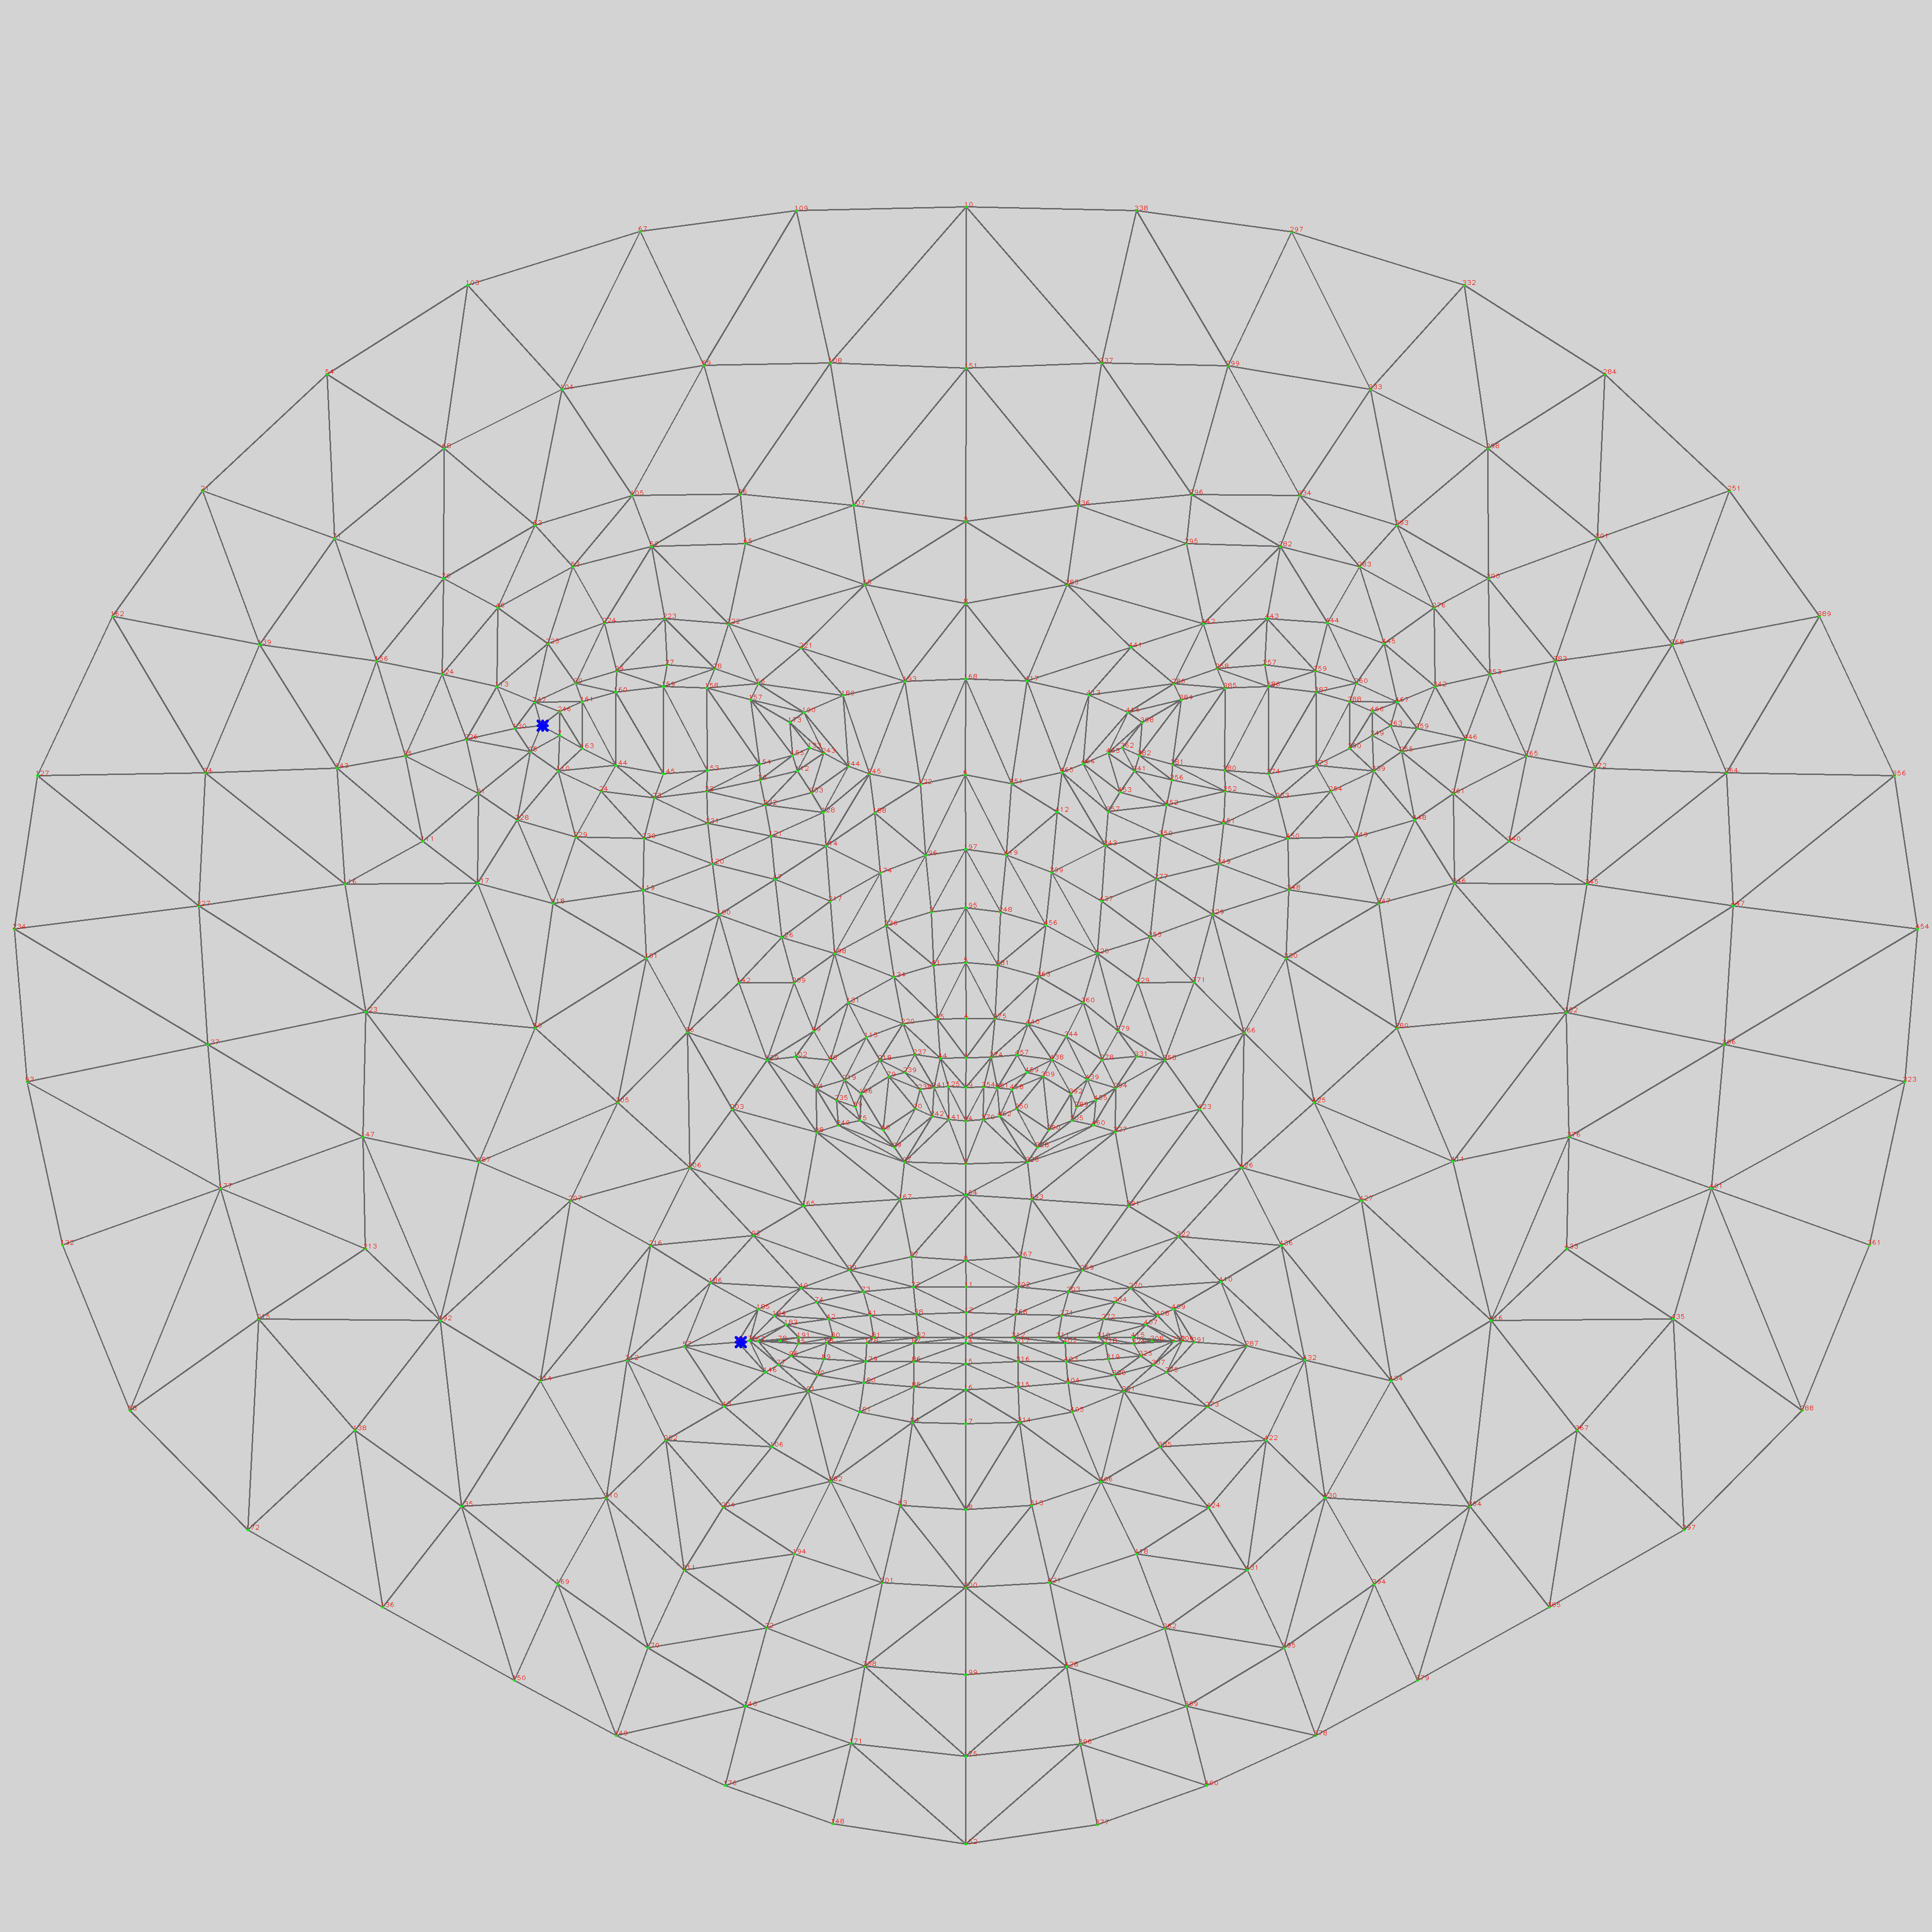
\includegraphics[scale=0.07]{figures/test.png}
    \caption{facemeshの特徴点}
    \label{one}
  \end{center}
\end{figure}
\\
\subsection{実行結果}
\subsubsection{入力画像}
入力として、今回は\hyperref[two]{図\ref{two}}、\hyperref[three]{図\ref{three}}の2枚の画像を用いた。
\begin{figure}[!ht]
  \begin{tabular}{cc}
    \begin{minipage}[t]{0.45\hsize}
      \centering
      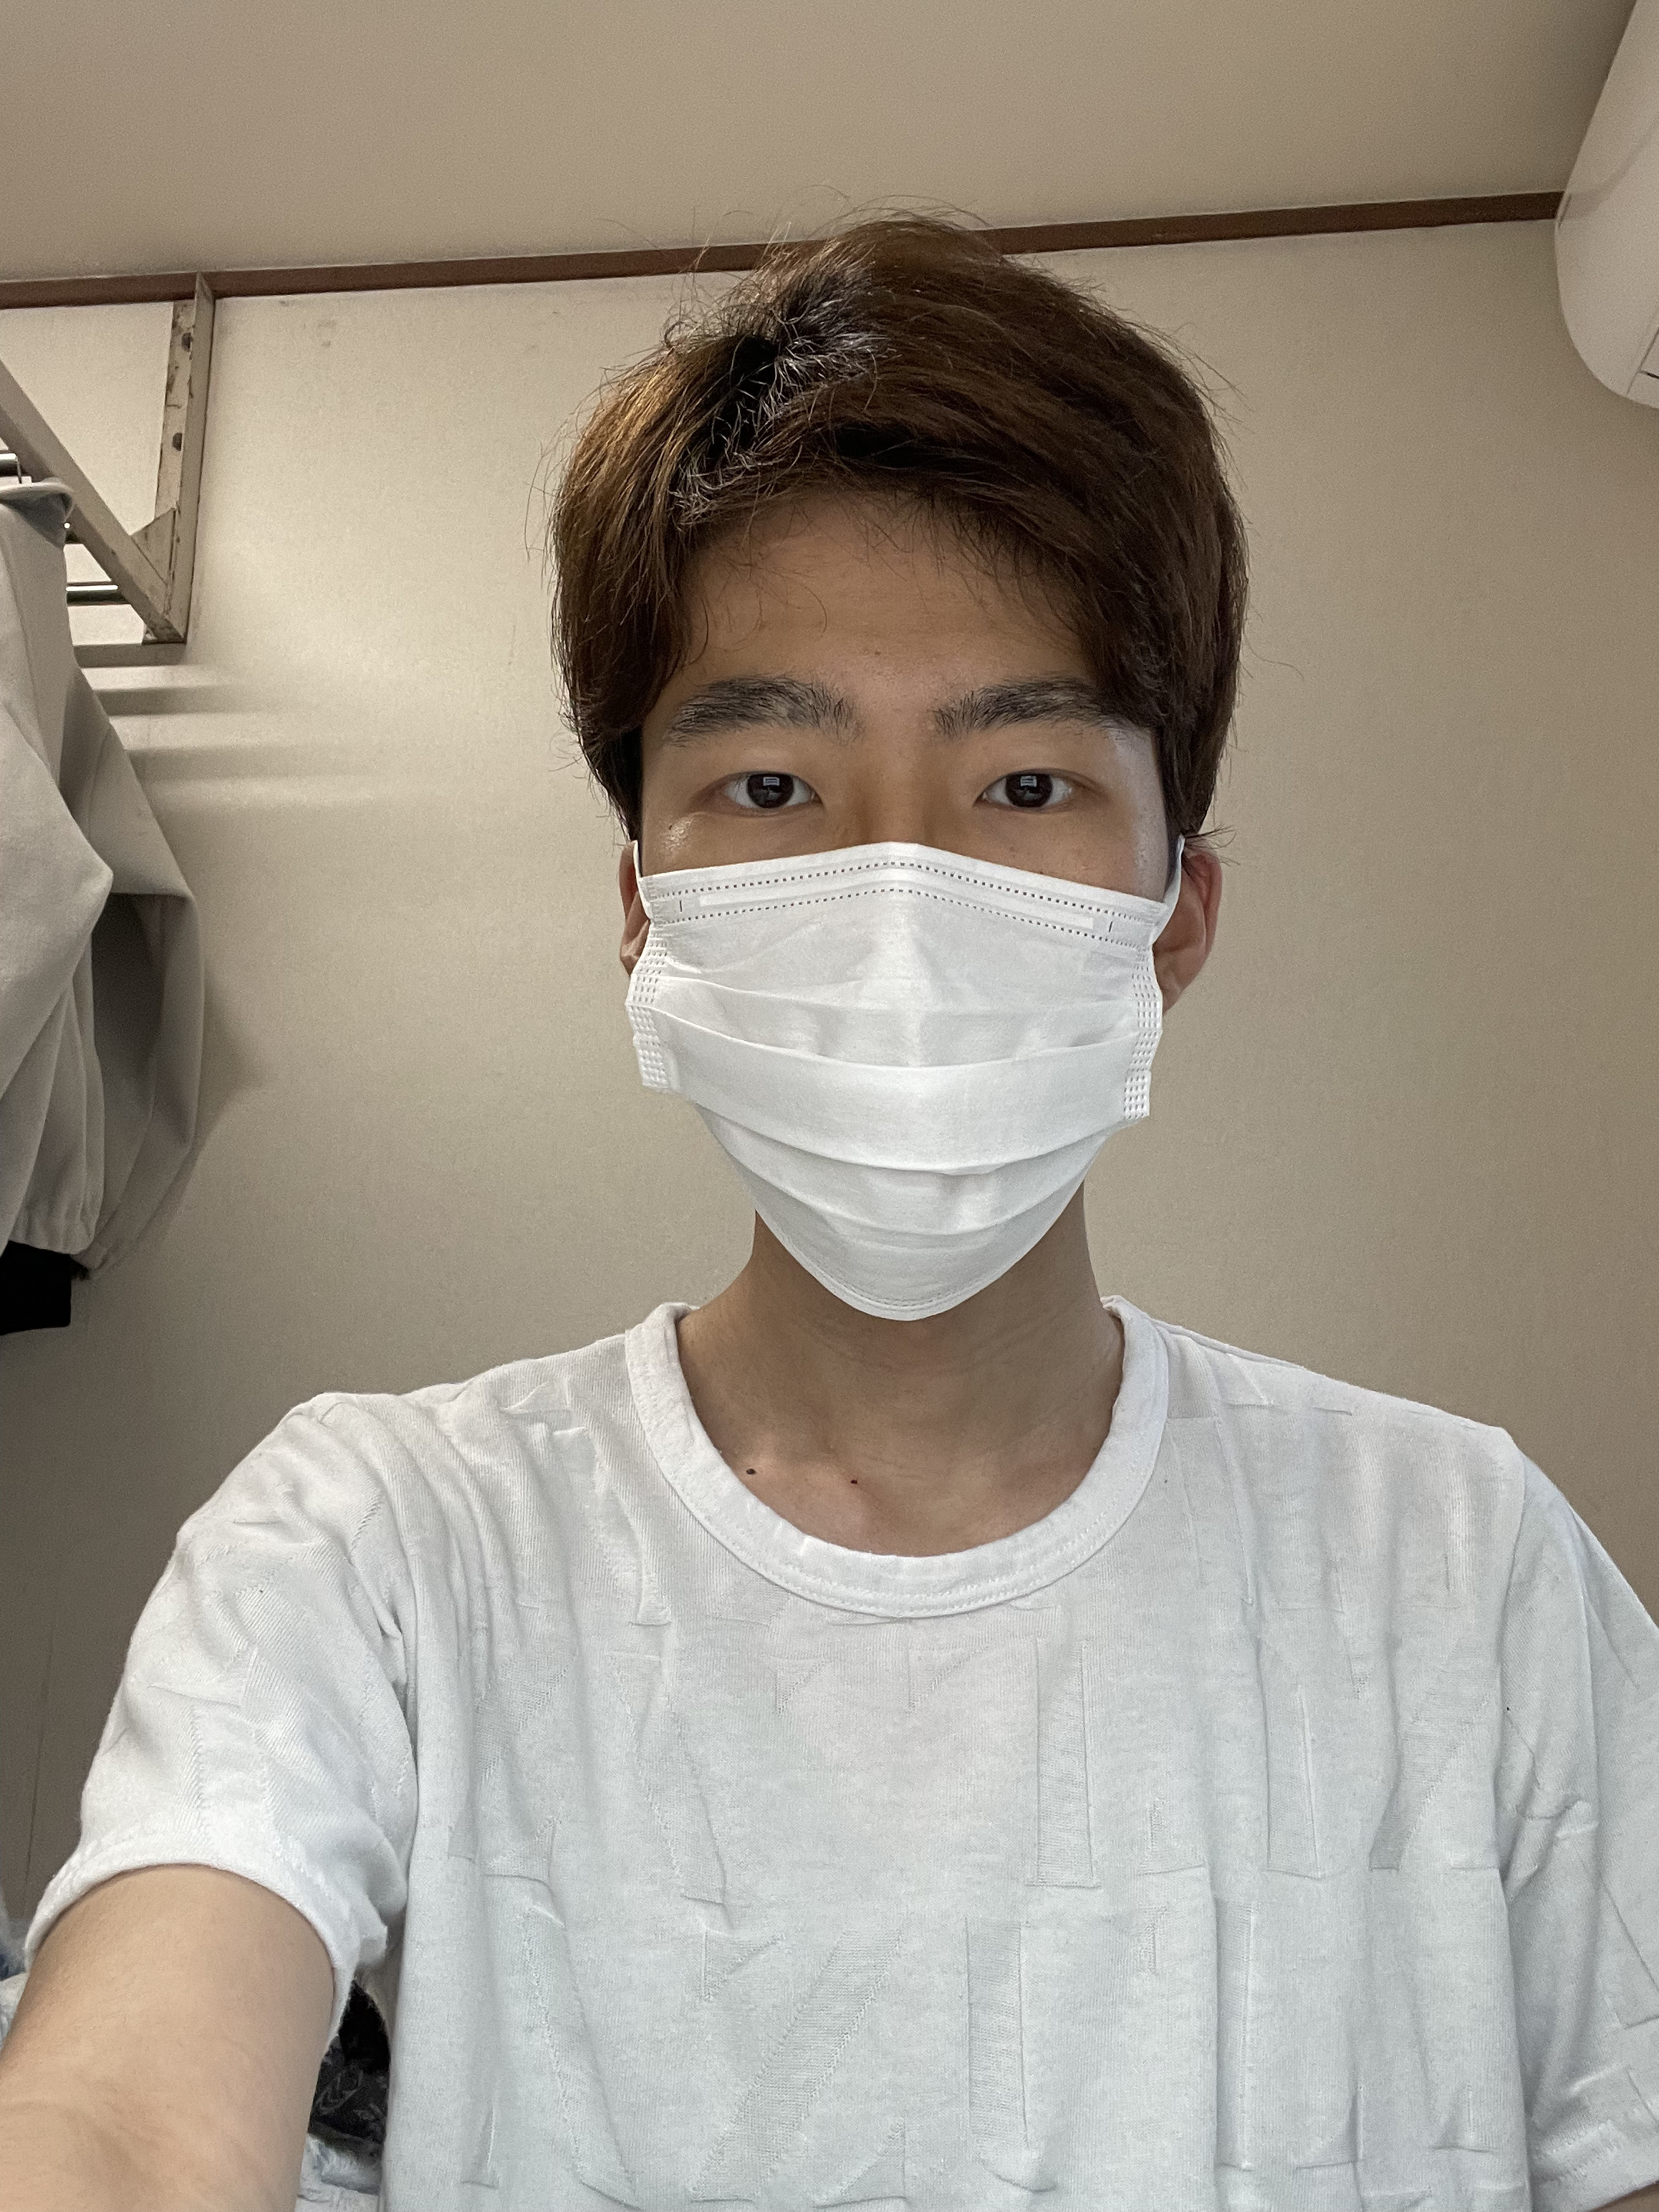
\includegraphics[keepaspectratio, scale=0.1]{figures/mask.jpg}
      \caption{マスクあり入力画像}
      \label{two}
    \end{minipage} &
    \begin{minipage}[t]{0.45\hsize}
      \centering
      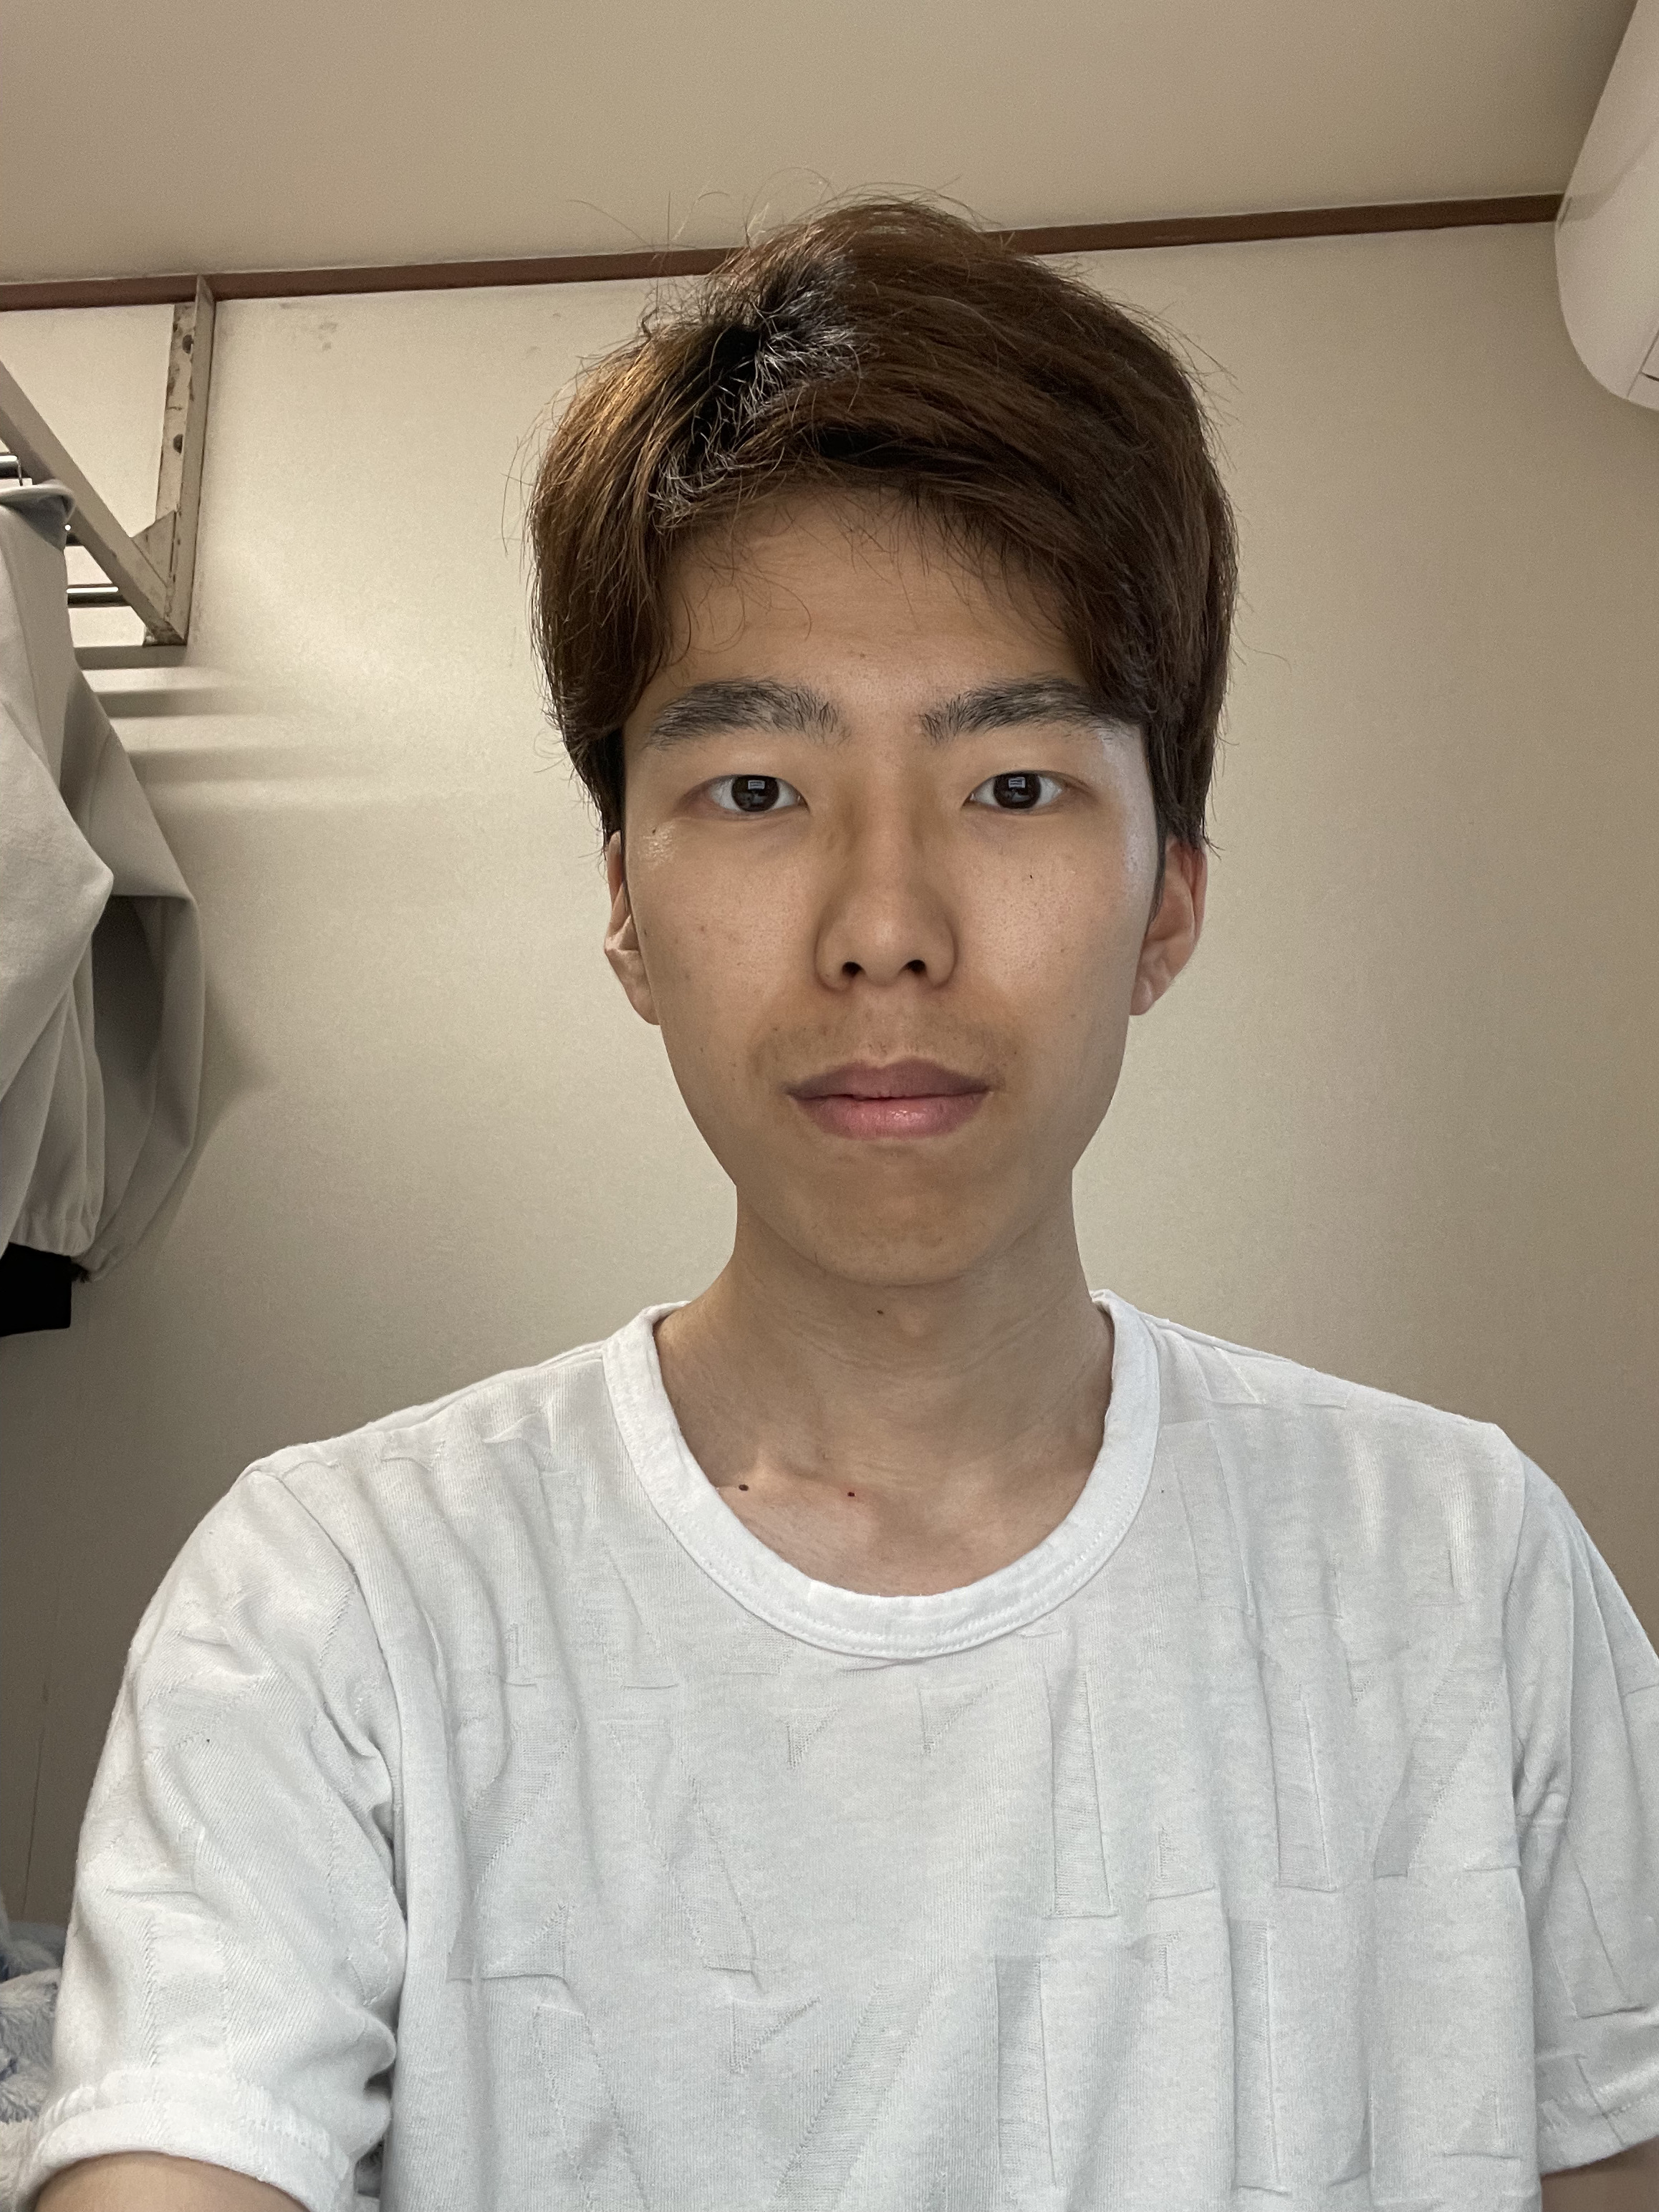
\includegraphics[keepaspectratio, scale=0.1]{figures/nomask.jpg}
      \caption{マスクなし入力画像}
      \label{three}
    \end{minipage}
  \end{tabular}
\end{figure}
\\
\subsubsection{出力画像}
出力された特徴点は\hyperref[four]{図\ref{four}}、\hyperref[five]{図\ref{five}}である。
\begin{figure}[!ht]
  \begin{tabular}{cc}
    \begin{minipage}[t]{0.45\hsize}
      \centering
      \includegraphics[keepaspectratio, scale=0.1]{figures/face_mesh_mask.png}
      \caption{マスクあり入力画像の特徴点}
      \label{four}
    \end{minipage} &
    \begin{minipage}[t]{0.45\hsize}
      \centering
      \includegraphics[keepaspectratio, scale=0.1]{figures/face_mesh_nomask.png}
      \caption{マスクなし入力画像の特徴点}
      \label{five}
    \end{minipage}
  \end{tabular}
\end{figure}
\\
また、特徴点の範囲と、座標の比較は\hyperref[six]{表\ref{six}}に示す。
\begin{table}[h]
  \centering
  \caption{特徴点の比較}
  \label{six}
  \begin{tabular}{|c|c|c|c|c|c|}
      \hline
       & X範囲 & Y範囲 & Z範囲 & 61番の特徴点 & 33番の特徴点 \\ \hline
      マスクあり画像 & 756.36 & 814.74 & 543.62 & (1112.53, 1447.08, 9.28) & (998.15, 1105.07, 61.89) \\ \hline
      マスクなし画像 & 760.09 & 961.53 & 582.25 & (1116.97, 1520.36, 12.13) &  (978.31, 1116.58, 56.31) \\ \hline
  \end{tabular}
\end{table}
\\
X座標の範囲はマスクの有無によって大きな差は出なかったが、YおよびZ座標の範囲には大きな差が出た。
Y座標の範囲に大きな差が出た原因は、マスクをしている場合、あごの下の位置を識別することができていないからだと、出力座標を見ても考えられる。
また、Z座標の範囲に大きな差が出た原因は、マスクをしている場合、Z座標の基準になる頭の中心の座標がうまく求めれず、全体的にずれてしまったからではないかと考えられる。\\
また61番の特徴点の座標(マスクで隠れる部分)を比較すると、やはりX座標はある程度正確だが、Y座標が大きく異なっていることがわかる。
Z座標については61番の特徴点と33番の特徴点でどちらも同じくらい異なっている。マスクがあることでZ座標の基準がずれてしまっていることがここからも考えられる。\\
\section{三次元モデルの修正}
三次元モデルが顔上の特徴点に合うようにモデルそのものの変更と、モデルスケールの変更、モデル位置の変更を行った。

\subsection{mqo形式にモデルを変更}
以前作成した三次元顔モデルはobj形式で、今利用している三次元モデルをfacemeshの特徴点に合わせて表示するプログラムではそのまま読み込むことができなかったので、mqo形式に変更した。
Windowsで三次元モデル作成ソフトのメタセコイアを用いてテクスチャを張り付ける必要がある。今回は、以下の手順でmqoファイルに変換した。
\begin{enumerate}
  \item obj形式でファイルをインポート
  \item 材質パネルで[新規]を選択
  \item 材質設定を開き[模様]を選択、uv展開されたテクスチャ画像を選択
  \item shiftキーを押しながらオブジェクトをクリックしオブジェクトの全体を選択
  \item タブの[選択部処理]を選択、[面に現在の材質を指定]を選択。
\end{enumerate}
ただ、このままではmqoファイルはプログラムで読み込むことができなかった。読み込むことができなかった原因は、メッシュが三角形メッシュと四角形メッシュで異なっていたからである。
三角形メッシュは四角形メッシュに比べて演算数が小さくなり、計算が速くなることがある。しかし、複雑な形の造形には不向きである。
Blenderを用いて三角形メッシュにモデルを変更し再度mqoファイルに変換することで、モデルが読み込むことができた。

\subsection{三次元モデルのスケールを変更}
3次元モデルのスケールを、顔の特徴点のスケールと同じになるように変更した。
3次元モデルのスケールはモデルのサイズと顔上の特徴点のサイズの比で求められる。実装の手順を下に示す。
\begin{enumerate}
  \item mqoファイルを読み込む際、モデルの$X,Y,Z$座標の最大値と最小値の差をモデルのサイズとしてセットする処理を追加
  \item 顔の特徴点を求める際、特徴点の$X,Y,Z$座標の最大値と最小値の差を顔のサイズとしてセットする処理を追加
  \item 顔のサイズをモデルのサイズで割った値をモデルのスケールと設定
  \item カメラのスケールを変更するOpenGLの関数であるglScalef()の引数をこの値に変更。
\end{enumerate}
なお、モデルのスケールを変更するのではなく、カメラのスケールを変更している。カメラの倍率や位置を変換することを視界変換、
カメラが見ているモデルの倍率や位置を変換することをモデリング変換というが、今回の場合はどちらの変換も同じ結果が得られる\cite{bib_1}。
\subsection{三次元モデルの位置を変更}
3次元モデルの位置を、顔の特徴点の位置と同じになるように変更した。3次元モデルが記述される世界座標系は、顔の特徴点の0番(鼻の上部)を原点として描かれる。
そのため鼻の上部の位置が原点になるようにモデルの位置を変更する必要がある。今回は、モデルの座標の平均が原点となるようにオフセットを設定する。実装の手順を以下に示す。
\begin{enumerate}
  \item mqoファイルを読み込む際、モデルの$X,Y,Z$座標の平均をモデルのオフセットとしてセットする処理を追加
  \item カメラの位置を動かすOpenGLの関数であるglTranslatef()の引数をこの値に変更。
\end{enumerate}

\subsection{実行結果}
Facemeshで得られた顔の特徴点を基に、三次元モデルを張り付けた画像のうち
スケール、位置を変更する前の出力画像を\hyperref[seven]{図\ref{seven}}に、変更した後の出力画像を\hyperref[eight]{図\ref{eight}}に示す。\\
\begin{figure}[!ht]
  \begin{tabular}{cc}
    \begin{minipage}[t]{0.45\hsize}
      \centering
      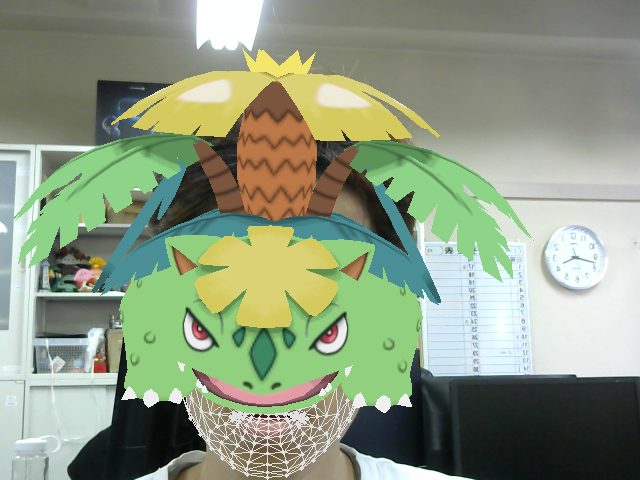
\includegraphics[keepaspectratio, scale=0.3]{figures/output1.png}
      \caption{変更前の出力画像}
      \label{seven}
    \end{minipage} &
    \begin{minipage}[t]{0.45\hsize}
      \centering
      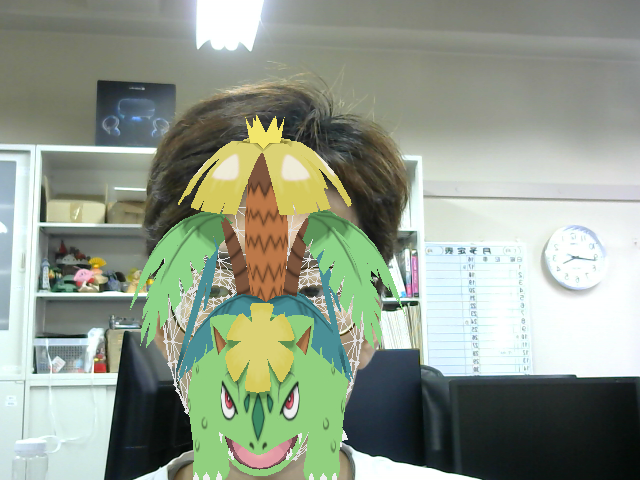
\includegraphics[keepaspectratio, scale=0.3]{figures/output2.png}
      \caption{変更後の出力画像}
      \label{eight}
    \end{minipage}
  \end{tabular}
\end{figure}
これを見ると、三次元モデルと特徴点がほぼ同じスケールになっていることが確認できる。また、位置もおおよそあっていることがわかる。
また、三次元モデルの向きについては途中で大きくずれてしまうことがある。原因について様々なモデルを使って調べたところ、特徴点のある部分と
三次元モデルを重複して描けないのが原因なのではと考えた。これについてはもう少し原因を究明していきたい。
\section{研究計画}
現時点で進行中の研究や、次回の発表時までに勧めたい研究計画を以下にまとめる。\\
\\
進行中
\begin{itemize}
  \item 顔上の特徴点を用いた類似研究の論文の査読
  \item Z方向を含めた正規化
\end{itemize}
次週以降
\begin{itemize}
  \item 3次元顔モデルの顔の向きの修正
  \item より軽量で、実験に適した三次元顔モデルの作成
  \item マスクあり顔画像を三次元モデルで補完するプログラムの実装
  \item テクスチャ画像を特徴点の座標に合わせて貼り付ける方法を調べる
\end{itemize}

%参考文献
\begin{thebibliography}{99}
\bibitem{bib_1} OpenGL入門/モデルビュー変換,http://wisdom.sakura.ne.jp/system/opengl/index.html,閲覧日2023/6/16
\end{thebibliography}

\end{document}
